\section{Introduction to Machine Learning}


Machine Learning: Field of study that gives computers the ability to learn without being explicitly programmed. \\

Well-posed Learning Problem: A computer program is said to learn from experience E with respect to some task T and some performance measure P, if its performance on T, as measured by P, improves with experience E. \\

Machine Learning Algorithms
\begin{itemize}
\item Supervised Learning
\item Unsupervised Learning
\item Reinforcement Learning
\item Recommender Systems
\end{itemize}


\subsection{Supervised Learning}

In supervised learning, we are given a data set and already know what our correct output should look like, having the idea that there is a relationship between the input and the output.\\

Supervised learning problems are categorized into "regression" and "classification" problems. In a regression problem, we are trying to predict results within a continuous output, meaning that we are trying to map input variables to some continuous function. In a classification problem, we are instead trying to predict results in a discrete output. In other words, we are trying to map input variables into discrete categories. \\

In \textbf{supervised learning}, the "right answers" are known.\\

A \textbf{Regression} is predicting a value! For example Given a picture of a person, we have to predict their age on the basis of the given picture\\

A \textbf{classification} is breaking into groups or discrete values.  For example Given a patient with a tumor, we have to predict whether the tumor is malignant or benign.\\


\subsection{Unsupervised Learning}

In \textbf{unsupervised learning}, the "right answers" are \textbf{not} known.\\



Unsupervised learning allows us to approach problems with little or no idea what our results should look like. We can derive structure from data where we don't necessarily know the effect of the variables.\\

We can derive this structure by clustering the data based on relationships among the variables in the data.\\

With unsupervised learning there is no feedback based on the prediction results. \\

\subsection{Model}

Input variables or input features are denoted as $x^{(i)}$\\
Output or target variable we are trying to predict are denoted as $y^{(i)}$\\
The pair $(x^{(i)}, y^{(i)})$ is called a training example.\\

To establish notation for future use, we’ll use $x^{(i)}$ to denote the \textbf{“input”} variables (living area in this example), also called input features, and $y^{(i)}$ to denote the \textbf{“output”} or target variable that we are trying to predict (price). A pair $(x^{(i)}, y^{(i)})$ is called a \textbf{training example}, and the dataset that we’ll be using to learn—a list of m training examples $(x^{(i)}, y^{(i)})$; i=1,...,m—is called a \textbf{training set}. Note that the superscript “(i)” in the notation is simply an index into the training set, and has nothing to do with exponentiation. We will also use \textbf{X} to denote the space of input values, and \textbf{Y} to denote the space of output values. In this example, X = Y = $\mathbb{R}$.

To describe the supervised learning problem slightly more formally, our goal is, given a training set, to learn a function
\begin{equation}
  h : X \rightarrow Y
\end{equation}
so that h(x) is a “good” predictor for the corresponding value of y. For historical reasons, this function h is called a hypothesis. Seen pictorially, the process is therefore like this:

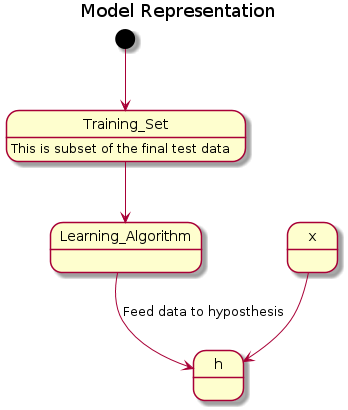
\includegraphics{model_representation.png}

When the target variable that we’re trying to predict is continuous, such as in our housing example, we call the learning problem a regression problem. When y can take on only a small number of discrete values (such as if, given the living area, we wanted to predict if a dwelling is a house or an apartment, say), we call it a classification problem. \\

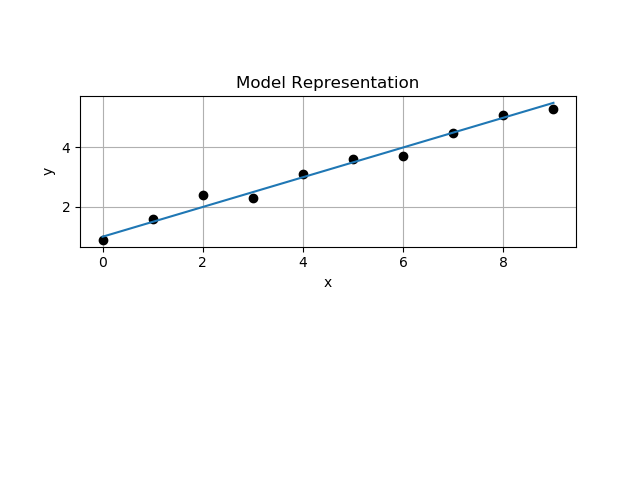
\includegraphics{python/model_plot_representation.png}\\

This is an attempt at a linear fit for this data.  It is not quite a match, but it is very close.  The plot for the line is $y=0.5x+1$ which is our hypothesis fuction h. 


\subsection{Cost Functions}

We can measure the accuracy of our hypothesis function by using a \textbf{cost function}. This takes an average difference (actually a fancier version of an average) of all the results of the hypothesis with inputs from x's and the actual output y's. \\

\begin{equation}
J(\theta_{0}, \theta_{1}) = \frac{1}{2m} \sum_{i=1}^{m} (\hat{y} -y^{i})^{2} = \frac{1}{2m} \sum_{i=1}^{m} (h_{\theta}(x^{i})-y^{i})^2
\end{equation}

m is the number of training examples. The goal is to minimize $J(\theta_{0}, \theta_{1})$.

To break it apart, it is $\frac{1}{2} \bar{x}$ where $\bar{x}$ is the mean of the squares of $h_{\theta}(x^{i}) -y^{i}$, or the difference between the predicted value and the actual value.\\

This function is otherwise called the \textbf{Squared error function}, or \textbf{Mean squared error}. The mean is halved $\frac{1}{2}$ as a convenience for the computation of the gradient descent, as the derivative term of the square function will cancel out the $\frac{1}{2}$ term. \\

For our previous example of $y=0.5x + 1$, we have $h_{\theta}(x^{i}) = \theta_{0} + \theta_{1}x^{i}$.  This leads to our cost function of 

\begin{equation}
J(\theta_{0}, \theta_{1}) = \frac{1}{2m} \sum_{i=1}^{m} (\theta_{0} + \theta_{1}x^{i} - y^{i})^{2} 
\end{equation}

Choose $\theta_{0}, \theta_{1}$ so that $h_{\theta}(x)$ is close to $y$ for training examples $(x,y)$\\

\textbf{KEY NOTE:} The cost function calculates a single value based on a specific $\theta_{0}, \theta_{1}$ pair.  It does not find the best $\theta_{0}, \theta_{1}$ values.  These values are supplied.  Gradient Descent is the process of finding the best $\theta_{0}, \theta_{1}$ values.

If we try to think of it in visual terms, our training data set is scattered on the x-y plane. We are trying to make a straight line (defined by $h_{\theta}(x)$) which passes through these scattered data points.\\

Our objective is to get the best possible line. The best possible line will be such so that the average squared vertical distances of the scattered points from the line will be the least. Ideally, the line should pass through all the points of our training data set. In such a case, the value of $J(\theta_0, \theta_1)$ will be 0. 

\newpage
\begin{multicols}{2}
  [
    This is a cost function implementation for the simple linear equation of $h_{theta}(x) = \theta_{0} + \theta_{1}x$
  ]
  Matlab\\
  \matlabcode{matlab/cost_function.m}
  \columnbreak

  Python\\
  \pythoncode{python/cost_function.py}
  
\end{multicols}

\newpage
\begin{multicols}{2}
  [
    These are the test scripts for driving the cost\_function implementations.  Both are fed the same input data and come back with the same cost value of 0.019.
  ]
  Matlab\\
  \matlabcode{matlab/test_cost_function.m}
  \columnbreak

  Python\\
  \pythoncode{python/test_cost_function.py}
  
\end{multicols}

\newpage
\begin{multicols}{2}
  [
    This is an example of trying different values for $\theta_{0} and \theta_{1}$ and plotting the results.
  ]
  Matlab\\
  \matlabcode{matlab/plot_cost_function.m}
  \columnbreak

  Python\\
  \pythoncode{python/plot_cost_function.py}
  
\end{multicols}

This is the graph created by python, which looks better than the one from Matlab/Octave.  There are 3 line and circles for the actual data.  The first line is the blue one across the X-Axis since we are using 0,0.  The best fit line in red has the ideal value for minimizing cost.  The last line shows it being close, but a little off.\\

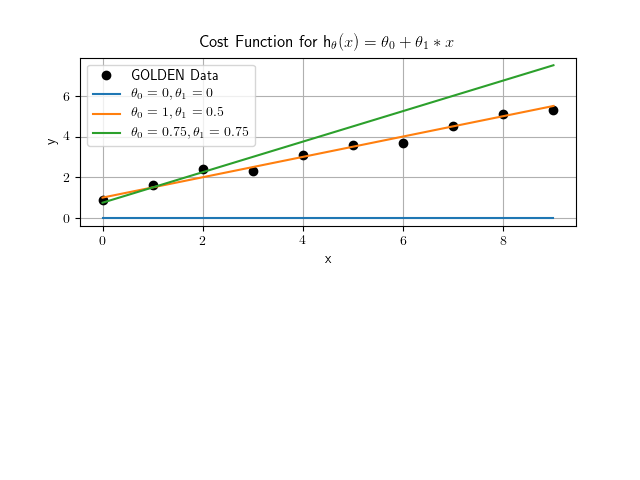
\includegraphics{python/plot_cost_function.png}\\

\subsection{Gradient Descent}

\textbf{KEY NOTE}: Gradient descent uses the hyposthesis function and cost function by iterating through various $\theta_0$ and $ \theta_1$ until it finds the minimum value for the cost function.  The $\theta_0$ and $ \theta_1$ for that position are the ones we want!\\

So we have our hypothesis function and we have a way of measuring how well it fits into the data. Now we need to estimate the parameters in the hypothesis function. That's where gradient descent comes in. \\

Imagine that we graph our hypothesis function based on its fields $\theta_0$ and $ \theta_1$ (actually we are graphing the cost function as a function of the parameter estimates). We are not graphing x and y itself, but the parameter range of our hypothesis function and the cost resulting from selecting a particular set of parameters. \\

We put $\theta_0$ on the x axis and $\theta_1$ on the y axis, with the cost function on the vertical z axis. The points on our graph will be the result of the cost function using our hypothesis with those specific theta parameters. The graph below depicts such a setup.\\

PUT GRAPH HERE

We will know that we have succeeded when our cost function is at the very bottom of the pits in our graph, i.e. when its value is the minimum. The red arrows show the minimum points in the graph.\\

The way we do this is by taking the derivative (the tangential line to a function) of our cost function. The slope of the tangent is the derivative at that point and it will give us a direction to move towards. We make steps down the cost function in the direction with the steepest descent. The size of each step is determined by the parameter $\alpha$, which is called the learning rate.\\

For example, the distance between each 'star' in the graph above represents a step determined by our parameter $\alpha$. A smaller $\alpha$ would result in a smaller step and a larger $\alpha$ results in a larger step. The direction in which the step is taken is determined by the partial derivative of $J(\theta_0,\theta_1)$. Depending on where one starts on the graph, one could end up at different points. The image above shows us two different starting points that end up in two different places. \\

The Gradient Descent Algorightm is:
\begin{equation}
  \theta_j := \theta_j - \alpha \frac{\partial}{\partial \theta_j} J(\theta_0, \theta_1)
\end{equation}

Repeat this until it converges!  Make sure to only update all $\theta$ values once all calculations are done.  We want to keep them constant while looping through everything.
\newpage
\begin{multicols}{2}
  [
    Gradient Descent Implementation
  ]
  Matlab\\
  \matlabcode{matlab/gradient_descent.m}
  \columnbreak

  Python\\
  \pythoncode{python/gradient_descent.py}
  
\end{multicols}

The cost function for a linear function is always bowl shaped on the 3d plot with a single global optima.

\subsection{Multivariate Linear Regression}

We want to predict the output \textit{y}.
We will have multiple features $x_{0}, x_{1}, x_{2} ... x_{n}$ where n is the number of features.
$x^{(i)}$ is the $i^{th}$ training example.
$x^{(i)}_{j}$ is the $i^{th}$ training example for feature j
m is the number of training examples.

Multivariate Linear Hypothesis is
\begin{equation}
  h_{\theta}(x) = \theta_{0} + \theta_{1} * x_{1} + \theta_{2} * x_{2} ... + \theta_{n} * x_{n}
\end{equation}

if we define $x_{0} = 1$ we can redfine the equation as 
\begin{equation}
  h_{\theta}(x) = \theta_{0}*x_{0} + \theta_{1} * x_{1} + \theta_{2} * x_{2} ... + \theta_{n} * x_{n}
\end{equation}

Which can be expressed as vectors $
\theta = 
\begin{bmatrix}
  \theta_{0} \\
  \theta_{1} \\
  \vdots    \\ 
  \theta_{n} \\
\end{bmatrix} $
and x = $
\begin{bmatrix}
  x_{0} \\
  x_{1} \\
  \vdots    \\ 
  x_{n} \\
\end{bmatrix} $

Which when put together in a linear algebra equation takes the form of
\begin{equation}
  h_{\theta}(x) = \Theta^{T}x
\end{equation}

In multivariate linear regression just multiple features in our linear regression to predict y.

\subsection{Gradient Descent for Multiple Variables}

hypothesis:  $h_{\theta}(x) = \theta_{0}*x_{0} + \theta_{1} * x_{1} + \theta_{2} * x_{2} ... + \theta_{n} * x_{n}$ \\

paramters: $\theta_{0}, \theta_{1} ... \theta_{n}$ \\

cost = $J(\theta_{0}, \theta_{1} ... \theta_{n}) = \frac{1}{2m} \sum_{i=1}^{m} (h_{\theta}(x^{i}) - y(i^{2}))^{2}$ \\

$J(\Theta)$ usually means the vector $\Theta$ \\

The process is to repeat until convergence.  We converge once the change in cost gets too small to really matter.
The general form for more than 1 feature is:
\begin{equation}
  \theta_{j} := \theta_{j} - \alpha *\frac{1}{m} \sum_{i=1}^{m} (h_{\theta}(x^{i}) -y^{i})*x_{j}^{i}
\end{equation}

This works out as:
\begin{equation}
  \begin{aligned}
  \theta_{0} := \theta_{0} - \alpha *\frac{1}{m} \sum_{i=1}^{m} (h_{\theta}(x^{i}) -y^{i})*x_{0}^{i} \\
  \theta_{1} := \theta_{1} - \alpha *\frac{1}{m} \sum_{i=1}^{m} (h_{\theta}(x^{i}) -y^{i})*x_{1}^{i} \\
  \theta_{2} := \theta_{2} - \alpha *\frac{1}{m} \sum_{i=1}^{m} (h_{\theta}(x^{i}) -y^{i})*x_{2}^{i} \\  
  \vdots \\  
  \theta_{n} := \theta_{n} - \alpha *\frac{1}{m} \sum_{i=1}^{m} (h_{\theta}(x^{i}) -y^{i})*x_{n}^{i} \\
  \end{aligned} 
\end{equation}

\subsubsection{Example}

Housing Data\\
\begin{tabular}{|c|c|c|c|c|}
  \hline
  Size & Bedrooms & Floors & Age & Price \\ \hline
  2104 & 5 & 1 & 45 & 460 \\ \hline
  1416 & 3 & 2 & 40 & 232 \\ \hline
  1534 & 3 & 2 & 30 & 315 \\ \hline
  852  & 2 & 1 & 36 & 178 \\ \hline
\end{tabular}
$
x^{2} = \begin{bmatrix}
  1416 \\
  3 \\
  2   \\ 
  40 \\
\end{bmatrix}
$ \\
$x_{3}^{2} = 2$

\subsection{Feature Scaling}

Idea: A problem with multiple features, make sure all features are on similar scales, Gradient Descent will converge more quickly.\\
EX:\\
$x_{1} $ = 0 - 2000 sq feet\\
$x_{2}$ = 1-5 bedrooms \\

These are very different ranges!  Contours of cost function take on a very skewed elliptical shape.  Can take a long time for gradients to find global minimum.

Scale features:\\
$x_{1} = \frac{size in feet^{2}}{2000}$\\
$x_{2} = \frac{number of bedrooms}{5}$

This puts everyone on a 0-1 scale so they are equally weighted.  Gradient descent should work quicker.

Generally want all features in a $-1 \leq x_{i} \leq 1$.  This is not a hard rule.  Should just be similar in scale.

\subsubsection{Mean Normalization}

Replace $x_{i}$ with $x_{i} - \mu_{i}$ to make features have approximately 0 mean.  Do \textbf{NOT} apply to $x_{0}$\\
EX:\\
$x_{1} = \frac{size-1000}{2000}$\\
$x_{2} = \frac{bedrooms - 2}{5}$\\
This puts $x_{1}$ and $x_{2}$ in between -0.5 and +0.5

$x_{i} = \frac{x_{i} - \mu_{i}}{s_{i}}$ Where $\mu_{1}$ is the average value and $s_{i}$ is the range or the standard deviation.

\subsection{Gradient Descent Learning Rate}

Plotting $J(\theta)$ vs number of iterations, as gradient descent runs, it should be decreasing on each iteration.  Once plot levels off, we have converged or are close enough.  The number of iterations is hard to predict could be 30 or 3,000,000 or more.  Automatic convergence tests are helpful.  If cost function decreases by some small $\epsilon$ like $10^{-3}$ in an iteration.  Finding this threshold is hard.\\

If $J(\theta)$ is increasing, gradient descent is not working and you should try a smaller $\alpha$\\

If $J(\theta)$ is bouncing up and down, it is not working and you should try a smaller $\alpha$\\

If $\alpha$ is too small, gradient descent will converge very slowly.\\

To choose $\alpha$ try 0.001, 0.01, 0.1, 1..... \\
Usually try 0.001, 0.003, 0.01, 0.03, 0.1, 0.3, 1 ...\\

\subsection{Features and Polynomial Regression}
Different learning algorithms based on different features.\\
Polynomial regression will let you fit non-linear functions.\\
Depends on insight in problem.\\

\subsubsection{Polynomial Regress}

If a linear fit does not appear to match data, you can use polynomials.
A quadratic function would look like this: $h_{\theta}(x) = \theta_{0} + \theta_{1}*x + \theta_{2}*x^{2}$
A cubic function would look like this: $h_{\theta}(x) = \theta_{0} + \theta_{1}*x + \theta_{2}*x^{2} + \theta_{3}*x^{3}$

\subsection{Normal Equation}

Normal equation is a method to solve for $\theta$ analytically instead of iteratively.  One step and it's done, no process or convergence.

Gradient descent gives one way of minimizing J. Let’s discuss a second way of doing so, this time performing the minimization explicitly and without resorting to an iterative algorithm. In the "Normal Equation" method, we will minimize J by explicitly taking its derivatives with respect to the $\theta$js, and setting them to zero. This allows us to find the optimum theta without iteration. The normal equation formula is given below:

\begin{equation}
  \Theta = (X^{T}X)^{-1}X^{T}y
\end{equation}

EX: For 1-D
$$
J(\theta) = a\theta^{2} + b\theta + c
\frac{d}{d\theta} J(\theta) = 2a\theta + b = 0 then solve for \theta
$$


EX: For more than 1-D
Take the partial for J for each $\theta$ , set to 0 and solve
\begin{equation}
  J(\theta_{0}....\theta_{m}) = \frac{1}{2m}\sum_{i=1}^{m} (h_{\theta}(x^{(i)}) - y^{i})^{2}
  \frac{\partial}{\partial \theta_{j}} = ... = 0 for each j solve for all the \theta values
\end{equation}
